\documentclass[a4paper, 14pt]{article}
\usepackage[utf8]{inputenc}
\usepackage{amsmath,amsfonts,amssymb,amsthm,mathtools} % AMS
\usepackage{wrapfig,lipsum, cleveref}
\usepackage{icomma} 
\usepackage{color}
\usepackage{geometry} 
\usepackage{longtable}
\usepackage{booktabs}

\linespread{1.5}

\geometry{top=25mm}
\geometry{bottom=35mm}
\geometry{left=35mm}
\geometry{right=20mm}


%% Номера формул
%\mathtoolsset{showonlyrefs=true} % Показывать номера только у тех формул, на которые есть \eqref{} в тексте.

%% Шрифты
\usepackage{euscript}	 % Шрифт Евклид
\usepackage{mathrsfs} % Красивый матшрифт

%% Свои команды
\DeclareMathOperator{\sgn}{\mathop{sgn}}

%% Перенос знаков в формулах (по Львовскому)
\newcommand*{\hm}[1]{#1\nobreak\discretionary{}
{\hbox{$\mathsurround=0pt #1$}}{}}


\title{Вариация алгоритма кросс-валидации со взвешиванием наблюдений}
\usepackage{cmap}					% поиск в PDF
\usepackage[T2A]{fontenc}			% кодировка
\usepackage[utf8]{inputenc}			% кодировка исходного текста
\usepackage[english,russian]{babel}	% локализация и переносы
\usepackage{graphicx}
\graphicspath{{pictures/}}
\DeclareGraphicsExtensions{.pdf,.png,.jpg}
\author{Гармидер Петр}
\date{\today}
\begin{document}


\thispagestyle{empty}
\begin{center}
	\textbf{ПРАВИТЕЛЬСТВО РОССИЙСКОЙ ФЕДЕРАЦИИ}\\
	\vspace{2ex}
	\textbf{Федеральное государственное автономное образовательное учреждение \\ высшего образования Национальный исследовательский университет \\ <<Высшая школа экономики>>}
	
	
	\vspace{8ex}
	
	\textbf{Факультет компьютерных наук}
\end{center}
\vspace{9ex}

\begin{center}
	{\textbf{КУРСОВАЯ РАБОТА
	}}
	\vspace{1ex}
	
	\underline{БАЙЕСОВСКИЙ ПОДХОД ДЛЯ АНАЛИЗА ДТП} \\
	\underline{BAYESIAN APPROACH TO CAR ACCIDENTS ANALYSIS}\\
	\vspace{1.5ex}
	
	по направлению подготовки \underline{01.04.02 Прикладная математика и информатика} \\
	образовательная программа \underline{<<Науки о Данных>>}
	
\end{center}
\vspace{1ex}
\begin{flushright}
	\noindent
	Студент группы АИД-Б20:\\Гармидер Петр Александрович\\
	\vspace{13ex}
	Научный руководитель:\\
	Борис Демешев
	
\end{flushright}	

\vfill

\begin{center}
	Москва 2021
	
\end{center}
\newpage

\tableofcontents

\newpage

\section{Введение}
\subsection{Актуальность в РФ} 
Транспорт является важной экономической и социальной составляющей жизни населения. Безопасность и эффективность транспортного передвижения непосредственно влияют на качество жизни. Пусть юридически, дороги могут находиться не только в государственной собственности, но и принадлежать частным, юридическим лицам, но по факту за качество и безопасность большей части дорог отвечает государство. Притом, у государства есть множество вариантов воздействия на дорожное движение: качество и расположение построенных дорог, инфраструктура прилагаемая к дорогам, установление и контроль скоростных режимов на разных участках дорог и т.д. 

Правительство Российской Федерации, понимая важность вопроса выше утверждает Стратегию безопасности дорожного движения в Российской Федерации на 2018 --- 2024 годы, где как раз подтверждается понимание государства о наличии связи безопастности движения и качестве жизни населения. Принятая стратегия, показывает, что вопрос с безопасностью дорожного движения в России остается  открытым.

Основываясь на данных карточек ДТП г. Москва за 2015-2020 года, можно заметить, что количество погибших в ДТП снижается из года в год  (рис. 1), несмотря на отсутствие какого либо тренда в количестве ДТП за указанные года (рис. 2). %До сих пор не понял как реферить рискнуки :)%

\begin{figure}[h]\label{ris: pog_dynamics}
	\center{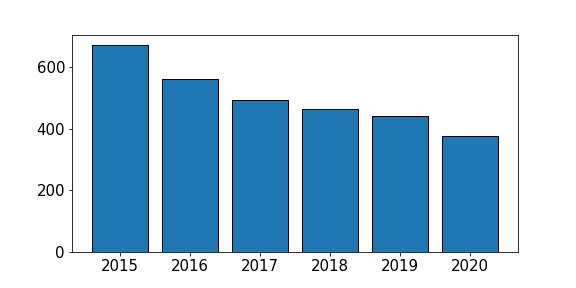
\includegraphics[scale=0.6]{img/pog_dyn_years}}
	\caption{Количество погибших в ДТП (г. Москва)}
\end{figure}

Как упоминается в \cite{kostych} согласно относительно свежим данным, есть несколько основных причин возникновения ДТП в РФ: 
\begin{itemize}
	\item нахождение детей на дороге или недалеко от нее
	\item загруженность дорог по выходным
	\item пренебрежение правилами дорожного движения водителем
	\item опрокидывание транспортного средства
	\item наезд на пешехода
\end{itemize}

Каждая вышеперечисленная причина в идеале требует отдельного анализа. Достаточно легко поверить, что не существует единого правила, которое способно ослабить риск каждого ДТП, однако верхнеуровневый анализ позволит понять некоторые самые <<проблемные>> места, работа над которыми даст максимальный эффект.

Наличие актуальной статистики дорожно-транспортных происшествий, в совокупности с анализом текущей ситуации позволит государству своевременно корректировать меры и действия в рамках принятой стратегии. 

\subsection{Обзор литературы}
Существует не так много статей посвященных анализу ситуации с ДТП в России. Основной причиной для этого считаю доступность и структурированность имеющихся данных. Существующие источники являются достаточно <<сырыми>>, что осложняет задачу для написания больших аналитических работ. Однако, исследования на эту тему все-таки есть.

В \cite{ivliev_econ_stat_analysis} авторы рассматривают дорожную ситуацию на верхнем уровне, оперируя федеральными округами и областями. Авторы подмечают важность плотности дорог (площадь на 1000 км территории). Наблюдается рост этого показателя во всей Российской Федерации, однако данный рост тяжело наблюдать оперируя отдельными федеральными округами. Из работы также можно понять, что в недалеком прошлом был небольшой ежегодный рост введения дорог с твердым покрытием. Авторы подмечают, что качество дорог является важный фактором не только для уменьшения количества инцидентов, но и для снижения степени тяжести ДТП. На уровень транспортных происшествий также влияет количество автомобилей. По данным на конец 2013 года в Российской Федерации насчитывалось порядка 53 321 тысяч транспортных средств, при росте в $17.5\%$ по отношению к прошлому году. Для того, чтобы оценить влияние количества транспортных средств на количество случае ДТП в статье строится регрессионная модель из которой следует, что это влияние действительно есть. Более того, количество автомобилей объясняют порядка $90\%$ дисперсии случаев ДТП по разным регионам. Статья в целом посвящена итогам Федеральной целевой программы по повышению безопасности дорожного движения в 2006---2012 гг. Авторы отмечают успех данной программы, но заявляют, что ситуация на дорогах все еще требует пристального внимания со стороны правительства.

Другая, достаточно свежая статья \cite{klachkiva2020analiz} посвящена анализу статистики ДТП на уровне всей страны. Авторы также отмечают бурный рост количества автомобилей зарегистрированных в РФ, что конечно ведет к дополнительным транспортным проблемам: снижение скорости сообщения из-за большей дорожной загрузки, увеличение выбросов вредных веществ, а также перерасход топлива. В своей работе, авторы делят пострадавших в ДТП по годам и подмечают, что не смотря на то, что общее количество ДТП и пострадавших в них уменьшается за последние 5 лет, существует рост количества пострадавших/погибших в ДТП детей в возрасте до 16 лет. Также авторы подмечают, что самая частая группа пострадавших в ДТП --- это люди с активным образом жизни от 21 до 40 лет. Такая ситуация, по словам авторов негативно сказывается на возрастную пирамиду населения и другие демографические показатели РФ. Авторы в своей работе отмечают снизившееся количество случаев ДТП в первую половину 2020 года, объясняя это снизившимся числом автомобилей на дороге. Однако, совсем недавно в \cite{rbkNews} отметили, что этот эффект был временным и в итоге локдаун 2020-го года никак не повлиял на количество фатальных случаев в ДТП. Как отмечают в ГИБДД, несмотря на сокращение случаев в ДТП, смертность в них, как и ситуация с вождением стала <<нестабильной>>\footnote{Стоит понимать, что данные могут разнится. В Российской Федерации актуальную информацию о случаях ДТП собирают два ведомства --- Госавтоинспеция и Росстат.}. По мнению службы, водители вновь севшие за руль после локдауна растеряли свои навыки вождения, а некоторые --- и чувство опасности, подавшись эйфории после ослабления некоторых ограничений.

В другой работе \cite{kuzmenko2020analysis} затрагивался вопрос прогнозирования вероятности ДТП с участием пешеходов. Авторы располагали похожими данным, что использовались и в данном исследовании --- карточки ДТП скачанные из сайта stat.gibdd.ru. Авторы описывают методологию сбора и построения витрины данных для последующей подачи на вход моделям машинного обучения. В работе выделяются основные факторы, которые могут иметь предсказательную силу, а также тонкостям сбора подобных данных. В качестве прогнозной модели авторы советуют использовать реализацию градиентного бустинга над деревьями Catboost --- библиотека с открытым доступом, разработанный компанией Яндекс. В статье рассказываются преимущества над существующими реализациями, а также даются рекомендации по настройке параметров модели. Авторы подчеркивают <<несовершенство>> данных в карточках ДТП, которые могут быть результатом человеческих ошибок. В качестве основной мотивации для создания подобной модели, выделяется высокая доля наездов на пешеходов, где наблюдается наивысшее среднее количество пострадавших в ДТП. Остается за кадром построение модели, как и формальная постановка задачи.

В работе \cite{konyuhov2015analysis} производится анализ динамики пострадавших в ДТП. На момент исследования данных наблюдалось снижение количества пострадавших и погибших на существенных статистически значимых показателях. Авторы также приводят некоторую сводку информации по ДТП, в частности заявляя, что самыми опасными часами являются вечерние --- 30-35 \% ДТП случаются именно в этот промежуток времени. Подтверждающий эту статистику график можно увидеть в разделе обзора данных. 

Авторы довольно ранней работы \cite{elvik2007state} рассматривают основные практики 2000-ных годов для выявления особо опасных участков дорог. На тот момент, байесовские методы являлись основным подходом для этой задачи. Строилась некоторая модель, которая каждому участку дороги ставила в соответствие распределение количества аварий, травм, крупных происшествий и др. Полученные оценки распределений сопоставлялись с фактическими данными, после чего аномально высокие значения для выведенных распределений трактовались как проблемные места, требующие особого внимания. Ряд стран использовал схожую методологию с поправкой на вид модели, критические пороги для объявление участка дороги проблемным и подобные технические характеристики. Такой подход позволял выявлять подозрительные участки дороги, на которые впоследствии отправлялись специалисты для выявления возможной причины <<опасности>> участка дороги и её устранения. В работе рассматривают разные спецификации модели, а также особенности практического влияния результатов. Как говорится в статье, на тот момент байесовский подход являлся state-of-the-art методом для подобного рода задач.


\subsection{Методология и цели}
Основной целью данной работы не является построение особо сложных моделей с использованием байесовской методологии. Автор не является специалистом в столь широкой области, но делает всё для того чтобы поближе познакомиться со столь интересным методом обработки и анализа информации. Данная работа --- хороший тренажер чтобы изучить основные концепции байесовского подхода и его отличия от классических статистических методов. Помимо моделирования, ценность работы заключается в обзоре и анализе располагаемых данных: поиск аномалий, выявление закономерностей, распознание общей динамики и тому подобное. Этой части в работе будет посвящена отдельная секция, большую часть которой будут занимать графики.

Работа рассматривается, как учебное упражнение, в связи с чем её результаты не рекомендуются к использованию для принятия каких-либо практических решений. 

Дополнительную ценность работе дает тот факт, что не существует популярных статей посвященных анализу дорожно-транспортных происшествий основанный на карточках ДТП с сайта Госавтоинспекции. 

Для количественного анализа будут использованы агрегированные данные по дням ДТП для дальнейшего выявления влияния различных погодных или сезонных условий на количество происходящих происшествий в отдельно выбранный день. В качестве модели будет использована классическая байесовская регрессия и представлены вероятностные интервалы для полученных апостериорных распределений коэффициентов на основе которых будут сделаны качественные выводы.

Совершенно очевидно, что не стоит ожидать каких-либо принципиально новых открытий сделанных байесовским подходом в сравнении с классическими частотными методами. Более того, достаточно известный факт, что задача байесовской регрессии, при определенных предпосылках на распределения неизвестных параметров, является одной из интерпретаций стандартных таких техник регуляризаций, как Lasso и Ridge \cite{haitovsky1980generalized}. Поэтому, еще раз подчеркивается, что нет особых явных указателей на то, что в рассматриваемой задачае байесовский подход является явно лучшим вариантом в сравнении с классическим частотным.

\section{Данные}
\subsection{Обзор}
Как уже говорилось ранее, не существует актуальных источников по дорожно-транспортным происшествиям в которых данные хранились бы в структурированном виде с возможностью дальнейшей обработки. Открытые для общего пользования ресурсы предоставляют доступ к слабоструктурированным данным за какой-то короткий промежуток на котором тяжело построить дальнейший анализ. Имеющиеся данные были получены благодаря Елене Никитиной, написавшей и выложившей в открытый доступ скрипт позволяющий получить данные по карточкам ДТП за любой доступный период в разрезе по регионам в машиночитаемом формате \cite{eleneGithub}. Непосредственным поставщиком данных является сайт stat.gibdd.ru --- официальный сайт Госавтоинспекции.

При помощи парсера были собраны данные по дорожно-транспортным происшествиям в г. Москва за промежуток с 2015 по 2020 года. Одно наблюдение --- карточка ДТП в которой указана информация заполненная инспектором ГИБДД приехавшим на место происшествия. Основные поля карточки ДТП включают в себя: идентификационный номер, дату, время, место происшествия, количество погибших и пострадавших в ДТП, информация по транспортным средствам, погодные условия, состояние покрытия дороги, данные об освещенности места ДТП, приблизительные координаты и некоторая обезличенная информация о погибших или раненных в инциденте. Стоит понимать, что каждый кусок данных уязвим к человеческим ошибкам и подвержен оценочному суждению, однако несет в себе какую-то информацию доступную для анализа. Почти все описанные поля принимают либо целочисленные значения, либо категориальные.

Также в открытом доступе удалось найти статистику по температуре в городе Москва\footnote{В аэропорту Шереметьево. Предполагается, что температура различалась не сильно.} в разрезе каждого дня. 

\subsection{Графический анализ данных}

\begin{figure}[h]
	\center{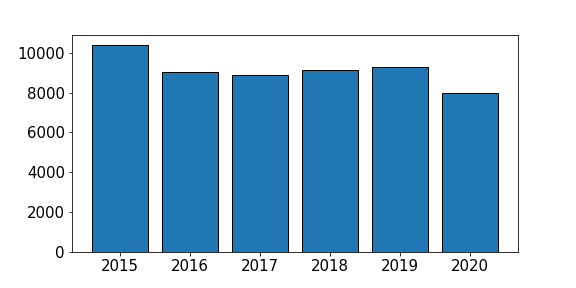
\includegraphics[scale=0.6]{img/dtp_count_years}}
	\caption{Общее количество случаев ДТП (г. Москва)}
\end{figure}

В данной секции будет сделан иллюстративный обзор данных в попытке запечатлеть некие закономерности и паттерны которые удалось выявить и изобразить на данных. 

На рис. 2 изображено количество всех случаев ДТП в г. Москва в разрезе по годам. Как видно из графика, начиная с 2016 года, строгого тренда не наблюдается. Явно выделяется результат введения ограничений в связи с COVID-19 в 2020 году, который привел к уменьшению дорожного поток, а вследствие чего к снижению вероятности возникновения ДТП. К сожалению, как уже говорилась ранее, данное наблюдение не согласуется с \cite{rbkNews}, однако может быть объяснено наличием разных источников данных. 

\begin{figure}[h]
	\center{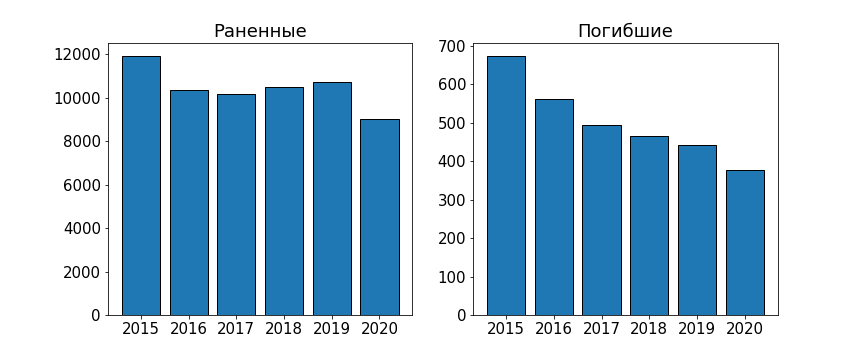
\includegraphics[scale=0.55]{img/ran_pog_years}}
	\caption{Количество раненных/погибших (г. Москва)}
\end{figure}

Также интересно посмотреть на динамику по пострадавшим в ДТП по годам. Можно увидеть, что количество раненных примерно совпадает с динамикой общего количества случаев ДТП (рис. 2). Однако количество погибших в ДТП падает из года в год. Невооруженным глазом видно, что это падение достигается не за счёт снижения динамики случаев ДТП. Однако, чтобы в этом точно убедиться можно посмотреть на рис. 4. Видим, что отношение количества раненных в ДТП к общему количеству зарегистрированных случаев примерно одинаковое от года к году. Однако, наблюдается снижение отношения погибших к количеству случаев на протяжении всего рассматриваемого периода.  Спад сходит на нет в 2020 году, что может быть объяснено неосторожностью вождения после отмены локдауна \cite{rbkNews}. 

\begin{figure}[h]
	\center{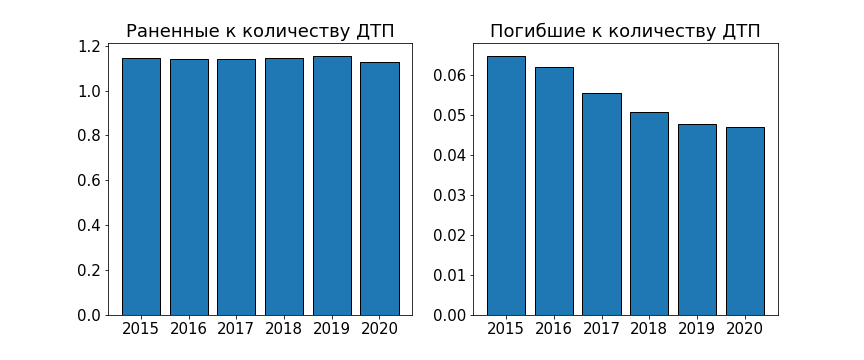
\includegraphics[scale=0.55]{img/ran_pog_ratios_years}}
	\caption{Отношение раненных/погибших к общему количеству ДТП (г. Москва)}
\end{figure}


Для общего контекста полезно понимать распределение погибших/раненных в ДТП за рассматриваемый период. Как и ожидалось, в случившимся ДТП в большинстве своем существует минимум один пострадавший. Любой сдвиг из этой точки большая редкость. С распределением погибших ситуация схожая с разницей в том, что мода количества погибших в ДТП находится в нуле. Данная картина не должна успокаивать, ибо это достаточно высокие цифры в перерасчете на количество населения. Есть некоторая статистика, которая показывает что в некотором наборе стран Россия занимает второе место по количеству погибших в ДТП на 100 тысяч населения \cite{tass_rating}. 

\begin{figure}[h]
	\center{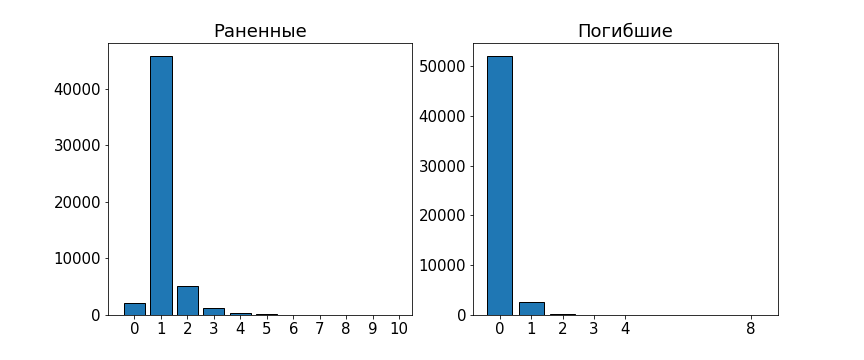
\includegraphics[scale=0.55]{img/ran_pog_hist}}
	\caption{Гистограммы раненных/погибших (г. Москва)}
\end{figure}

Для лучшего понимания дорожной ситуации можно также обратиться к похожим данным в разрезе по месяцам. На рис. 6 наблюдается явная закономерность показывающая, что количество ДТП, как и их тяжесть усугубляется к концу года. Причем количество раненных в ДТП резко увеличивается начиная с августа, что может быть объяснено через ухудшающаяся погоду к концу года, что приводит к ухудшению управляемости транспортного средства. Резкое падение в январе можно связать с низкой дорожной активностью в этот месяц. Также начало года выпадает на пик снежного сезона. Погодные условия способствуют снижению скоростного режима, что снижает риск и степень тяжести потенциальных ДТП.

\begin{figure}[h]
	\center{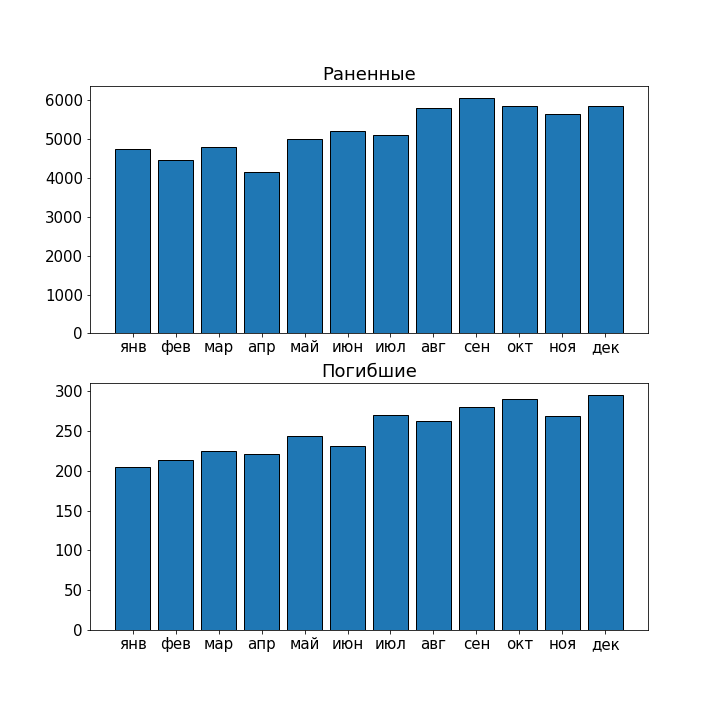
\includegraphics[scale=0.55]{img/ran_pog_month}}
	\caption{Динамика раненных/погибших по месяцам (г. Москва)}
\end{figure}

Для подробного рассмотрения вопроса о связи природных явлений и случаев ДТП полезно исследовать рис. 7. На данном графике отображена динамика количества погибших и раненных при ДТП в контексте средней температуры воздуха в рассматриваемый месяц. К сожалению обнаруживаем для себя, что явных закономерностей в какую-либо сторону выявить не удалось. Если всмотреться, то можно заметить, что данный график лишь повторяет динамику <<конца-начала>> года. Это дает основание считать, что погодные условия не являются важным драйвером к снижению уровня ДТП. Главным источником возможно является повышение активности на участках дорог в связи с наступающими новогодними праздниками в конце года и дальнейшее снижение активности водителей в связи с праздничными каникулами. 

\begin{figure}[h]
	\center{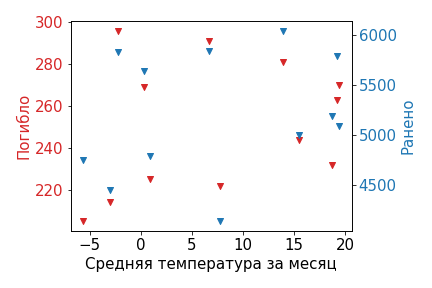
\includegraphics[scale=0.55]{img/ran_pog_temperature}}
	\caption{Динамика раненных/погибших в связке с средней температурой за месяц (г. Москва)}
\end{figure}

От месячного периода можно спустить на одну ступень ниже к разбиению по дням недели (см рис. 10). Можно сразу заметить, что выходные дни являются самыми опасными с точки зрения количества потенциальных в таких ДТП. Важно заметить, что пятница является самым популярным днем возникновения ДТП, однако остается <<безопасным>> в рамках среднего количества погибших. Возникает гипотеза о том, что большая доля жертв ДТП в субботу приходится на ночь с пятницы. Люди отдохнув в последний рабочий день, возможно в нетрезвом состоянии попадают в летальные ДТП. Это также описывает аномально высокую летальность субботы, как и низкую в пятницу. Воскресенье также является неблагоприятным днем, по всей видимости по тем же причинам, что и суббота. С высокой долей вероятности, такую картинку можно наблюдать не во всех регионах, а только в городах с развитым сервисом досуга, которым жители города и желают воспользоваться в свободный от работы день.

\begin{figure}[h]
	\center{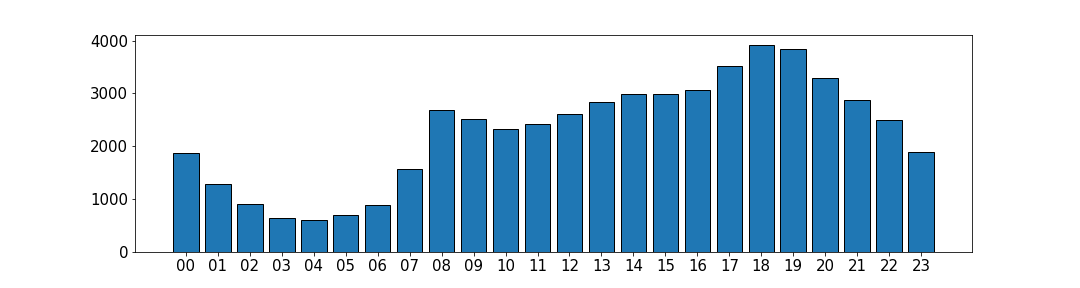
\includegraphics[scale=0.45]{img/dtp_count_hours}}
	\caption{Количество ДТП в разрезе часа дня (г. Москва)}
\end{figure}

Также интересно рассмотреть картину случаев ДТП в разрезе часов дня. Из рис. 8 можно подметить, что пиковые ситуации ДТП это начало и конец рабочего дня, причем ситуация более остро стоит в конец рабочей смены, возможно из-за накопленной в течении дня усталости и потери концентрации. Также довольно интересную картину можно наблюдать в разбиении на погибших и раненных (рис 9). На удивление, среднее количество раненных в ДТП почти не меняется от часа к часу, однако картина совершенно другая для летальных случаев. Наблюдаем резкий рост среднего количества погибших в ДТП после 12-ти часов ночи. На мой взгляд это не может быть объяснено освещением, т.к картина совершенно иная в 22-й и 23-й час. Одна из основных гипотез --- это сюжет, когда водитель или пешеход возвращается домой не в здравом рассудке (усталость или алкогольное опьянение). Ситуация явно <<стабилизируется>> в основные часы жизни население. Также возможно, высокая доля погибших в ночное время объясняется в трудностях в своевременном получении медицинских услуг. Конечно же, чтобы более аккуратно ответить на этот вопрос требуются дополнительные данные и отдельное исследование.

\begin{figure}[h]
	\center{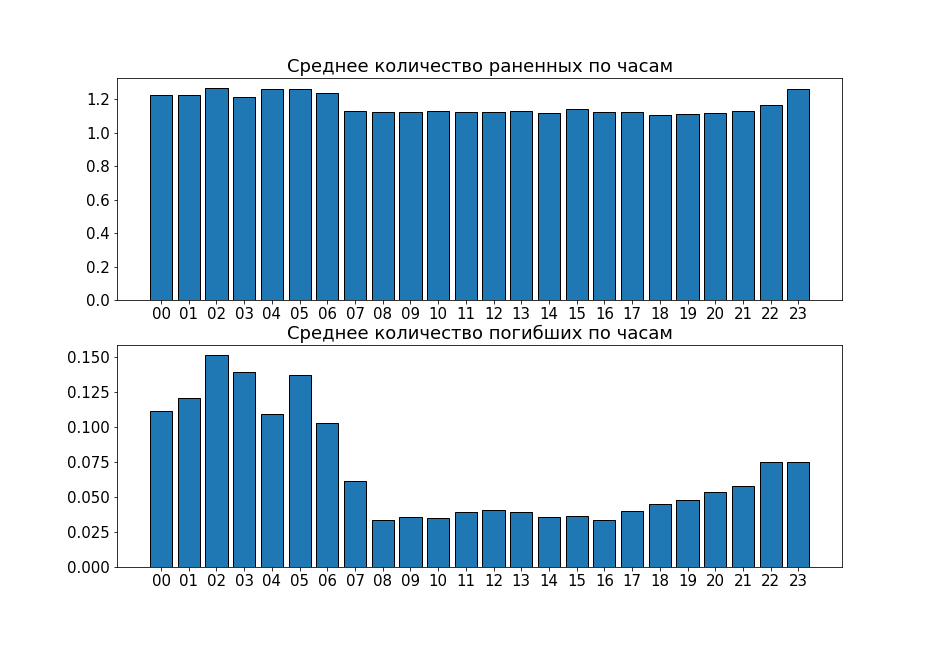
\includegraphics[scale=0.45]{img/ran_pog_mean_hour}}
	\caption{Среднее количество раненных и погибших по часам дня (г. Москва)}
\end{figure} 


\begin{figure}[h]
	\center{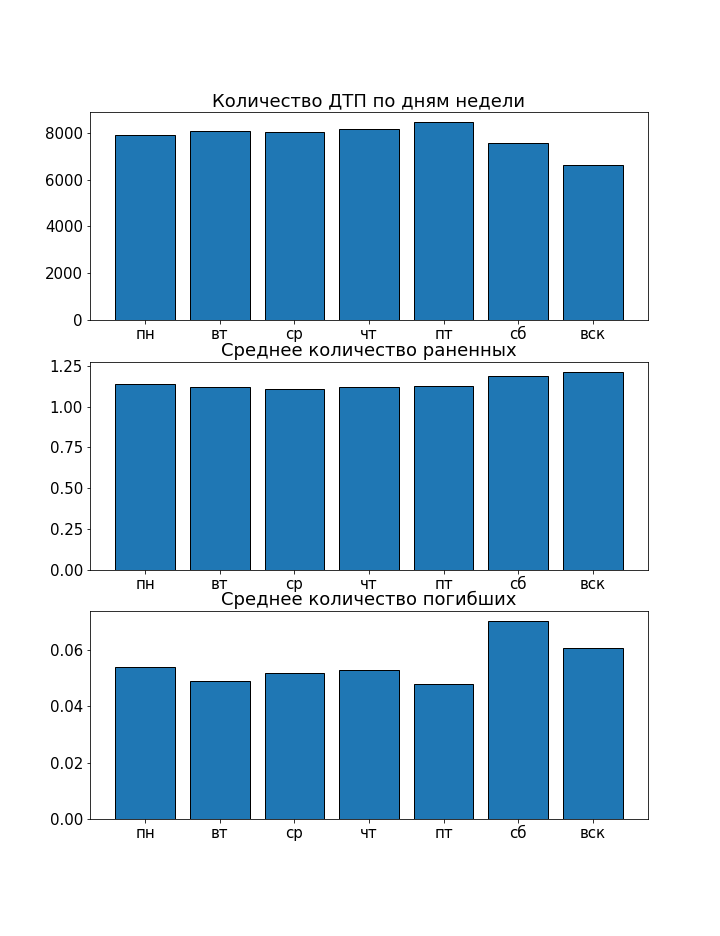
\includegraphics[scale=0.45]{img/ran_pog_ratios_weekday}}
	\caption{Среднее количество раненных и погибших по дням недели (г. Москва)}
\end{figure}

Для выявления общей динамики в течении года можно посмотреть на рис. 12, 13 и 14. Проявляется явная динамика ухудшения ситуации с дорожно-транспортными происшествиями от начала года к концу. На тепловой карте раненных в ДТП (рис. 12) явно выделяется апрель месяц. По каким-то причинам в это время присутствует временное падение случаев ДТП, как и количества раненных (рис. 6). Было достаточно тяжело определить возможную причину этого эффекта по имеющимся данным. Одно из возможных объяснений это сниженная дорожная активность в после режима самоизоляции в апреле 2020 года (рис. 11).

\begin{figure}[h]
	\center{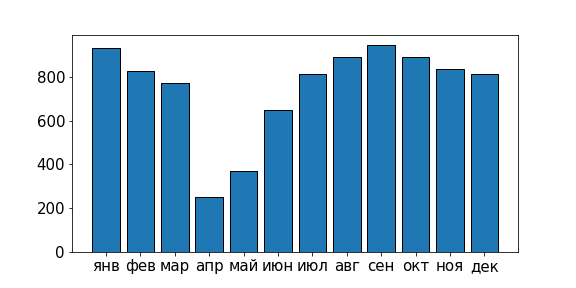
\includegraphics[scale=0.55]{img/2020_ran}}
	\caption{Количество пострадавших в ДТП 2020-й год (г. Москва)}
\end{figure}

\begin{figure}[h]
	\center{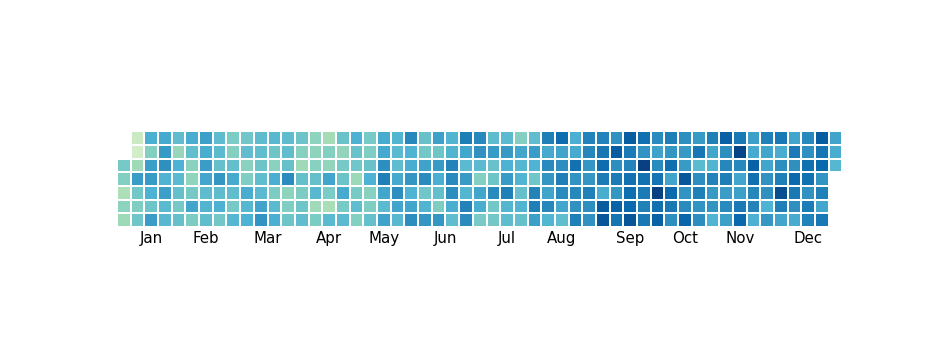
\includegraphics[scale=0.5]{img/dtp_count_heatmap}}
	\caption{Тепловая карта случаев ДТП (г. Москва)}
\end{figure}

\begin{figure}[h]
	\center{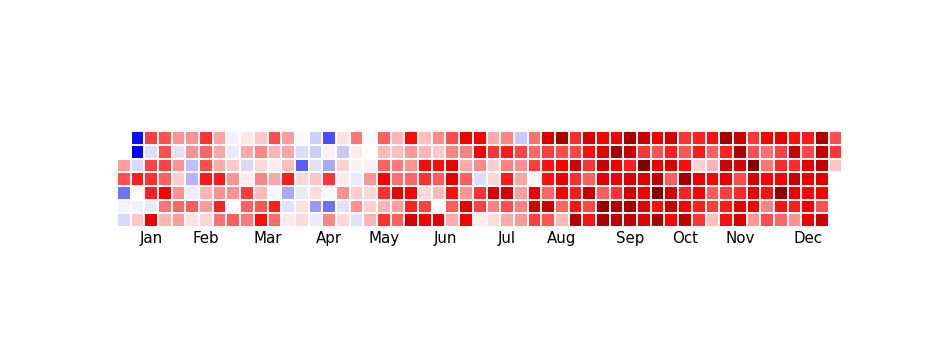
\includegraphics[scale=0.5]{img/dtp_ran_heatmap}}
	\caption{Тепловая карта раненных в ДТП (г. Москва)}
\end{figure}

\begin{figure}[h]
	\center{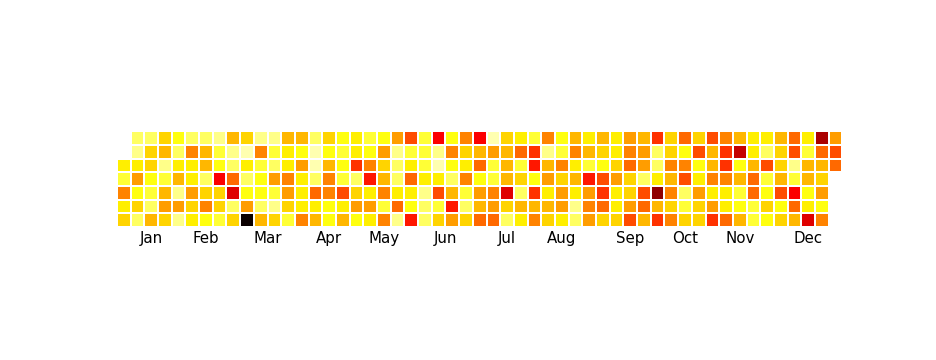
\includegraphics[scale=0.5]{img/dtp_pog_heatmap}}
	\caption{Тепловая карта погибших в ДТП (г. Москва)}
\end{figure}

На рис. 11 действительно можно видеть введение режима самоизоляции, как и его поэтапное ослабление с мая месяца. В этом контексте апрель больше не выглядит каким-то особенным <<безопасным>> месяцем, так как резкое снижение количества раненных в этом месяце (рис. 6) можно объяснить введением режима самоизоляции в этот период. Интересно, что локдаун\footnote{Ситуация в которой людям запрещено свободно перемещаться по городу в том числе с использованием транспортного средства.} никак не повлиял на количество погибших в апрель месяц 2020-го года. Скорее всего это объясняется тем, что большая часть ДТП с летальным исходом обусловлены особыми обстоятельствами участников ДТП и имеет слабую связь дорожным потоком. Действительно, как уже было видно на рис. 9, основная доля погибших приходится на ночное время с низкой загруженностью дорог. 	

Неспецифичность апреля месяца для степени тяжести ДТП можно видеть на рис. 14. В отличии от рис. 13, апрель не выделяется из общего тренда дорожно-транспортных происшествий, и с поправкой на количество случаев повторяет общую динамику частоты инцидентов. Тепловая карта ДТП (рис. 12) помогает убедиться в плавности учащение случаев ДТП из месяца в месяц, а в остальном повторяет агрегированную ежемесячную динамику.

На данный момент были выяснены основные сезонные и временные особенности дорожно-транспортных происшествий, а также эффект летальности данных показателей.  

\newpage
\noindent Основные выводы:
\begin{enumerate}
	\item В подавляющем большинстве случаев в ДТП есть один раненный 
	\item В подавляющем большинстве случаев в ДТП нет погибших
	\item Количество ДТП почти никак не изменяется из года в год
	\item Количество погибших в ДТП в расчете на один инцидент уменьшалось с 2015 по 2019 год
	\item Количество погибших в ДТП в расчете на один инцидент никак не изменилось в 2020 году по отношению к 2019 году
	\item Среднее количество раненных в ДТП никак не зависит от временных и сезонных особенностей инцидента 
	\item Количество случаев ДТП увеличивается к концу года, после чего резко падает в январе
	\item Температура воздуха слабо влияет на тяжесть ДТП, как и общую динамику в контексте месяцев
	\item Суббота и воскресенье являются самыми <<опасными>> днями, основываясь на среднем количестве погибших в ДТП в эти дни
	\item Большая часть ДТП происходит в рабочие часы с 8 утра до 10 вечера
	\item Большинство летальных случаев ДТП выпадает на ночное время 
	\item Режим самоизоляции уменьшил количество случаев ДТП, как минимум в апреле и мае месяцах (рис. 11)
	\item Режим самоизоляции никак не сказался на количестве летальных случаев в ДТП (рис. 15)
	\item Вопреки выдвинутой гипотезы об отсутствии связи летальности ДТП и уровня освещения дороги, связь была обнаружена (рис. 16)
	
\end{enumerate}

\begin{figure}[h]
	\center{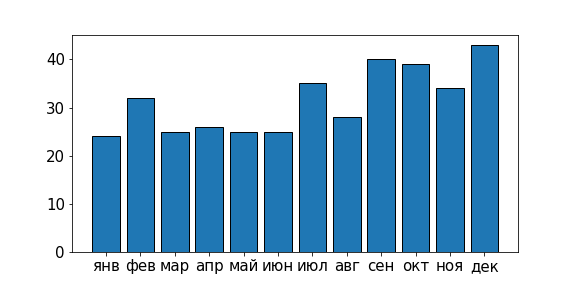
\includegraphics[scale=0.55]{img/2020_pog}}
	\caption{Количество погибших в ДТП 2020-й год (г. Москва)}
\end{figure}


\begin{figure}[h]
	\center{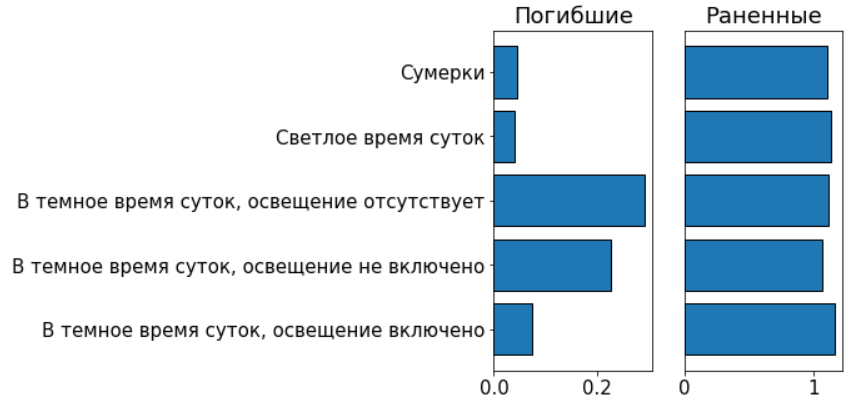
\includegraphics[scale=0.45]{img/pog_ran_osv}}
	\caption{Среднее количество погибших/раненных по типу освещения (г. Москва)}
\end{figure}



Упомянутая гипотеза об отсутствии влияния освещения на степень тяжести ДТП не подтвердилась. На рис. 16 видна явная связь этих показателей. Среднее количество погибших в ДТП гораздо ниже при наличии источников света. Видно, что в темное время суток при включенном освещении, среднее количество летальных случаев гораздо ниже ситуаций с отсутствием освещения и находится на уровне ДТП при естественных источниках света.

\section{Результаты модели и выводы}

Для моделирования использовалась стандартная байесовская регрессия. Модель выглядит следующим образом:

\[
	dtpCount_i = \beta_0 + \beta_1 temp_i + \sum_{j=2016}^{2020} \beta_{j - 2014}[year = j]_i + \sum_{j = 2}^{12} \beta_{j + 5} [month = j]_i +
\]
\[
	+ \sum_{j=1}^{6} \beta_{j + 17} * [weekday = j]_i
\]

\begin{table}[ht]
	\centering
	\begin{tabular}{rlrrrrrrr}
		\hline
		Parameter & Median & CI & CI\_low & CI\_high & pd & Rhat & ESS \\ 
		\hline
		Intercept) & 26.93 & 0.95 & 25.58 & 28.22 & 1.00 & 1.00 & 1502.94 \\ 
		temp & 0.26 & 0.95 & 0.21 & 0.32 & 1.00 & 1.00 & 1747.47 \\ 
		factor(year)2016 & -3.56 & 0.95 & -4.44 & -2.60 & 1.00 & 1.00 & 2889.02 \\ 
		factor(year)2017 & -3.85 & 0.95 & -4.79 & -2.95 & 1.00 & 1.00 & 2847.93 \\ 
		factor(year)2018 & -3.23 & 0.95 & -4.14 & -2.25 & 1.00 & 1.00 & 3052.08 \\ 
		factor(year)2019 & -3.17 & 0.95 & -4.08 & -2.25 & 1.00 & 1.00 & 2648.73 \\ 
		factor(year)2020 & -6.99 & 0.95 & -7.90 & -6.06 & 1.00 & 1.00 & 2605.14 \\ 
		factor(month)2 & 0.30 & 0.95 & -1.01 & 1.64 & 0.67 & 1.00 & 2015.02 \\ 
		factor(month)3 & -1.11 & 0.95 & -2.49 & 0.20 & 0.95 & 1.00 & 1672.39 \\ 
		factor(month)4 & -4.63 & 0.95 & -6.11 & -3.09 & 1.00 & 1.00 & 1471.72 \\ 
		factor(month)5 & -3.62 & 0.95 & -5.34 & -1.93 & 1.00 & 1.00 & 1287.39 \\ 
		factor(month)6 & -3.06 & 0.95 & -4.92 & -1.14 & 1.00 & 1.00 & 1315.87 \\ 
		factor(month)7 & -4.91 & 0.95 & -6.85 & -3.04 & 1.00 & 1.00 & 1309.13 \\ 
		factor(month)8 & -1.18 & 0.95 & -3.17 & 0.58 & 0.89 & 1.00 & 1272.19 \\ 
		factor(month)9 & 2.82 & 0.95 & 1.03 & 4.42 & 1.00 & 1.00 & 1340.43 \\ 
		factor(month)10 & 3.12 & 0.95 & 1.64 & 4.63 & 1.00 & 1.00 & 1466.13 \\ 
		factor(month)11 & 4.44 & 0.95 & 3.10 & 5.74 & 1.00 & 1.00 & 1715.74 \\ 
		factor(month)12 & 5.23 & 0.95 & 3.91 & 6.56 & 1.00 & 1.00 & 2015.89 \\ 
		factor(weekday)1 & 0.54 & 0.95 & -0.45 & 1.58 & 0.86 & 1.00 & 2588.40 \\ 
		factor(weekday)2 & 0.50 & 0.95 & -0.48 & 1.52 & 0.84 & 1.00 & 2580.39 \\ 
		factor(weekday)3 & 0.91 & 0.95 & -0.17 & 1.85 & 0.96 & 1.00 & 2250.87 \\ 
		factor(weekday)4 & 1.87 & 0.95 & 0.83 & 2.79 & 1.00 & 1.00 & 2258.78 \\ 
		factor(weekday)5 & -1.09 & 0.95 & -2.14 & -0.08 & 0.98 & 1.00 & 2654.72 \\ 
		factor(weekday)6 & -3.97 & 0.95 & -4.99 & -2.95 & 1.00 & 1.00 & 2437.26 \\ 
		\hline
	\end{tabular}
	\caption{Результаты модели}
\end{table}

Базовым годом был взят 2015-й. Базовый месяц --- январь. Базовый день недели --- понедельник. Коэффициенты при соответствующих факторных переменных следует интерпретировать относительно указанных базовых категорий.

В таблице 1 показаны результаты оценок распределений неизвестных коэффициентов стандартной байесовской регрессии: медиана, HPD\footnote{High probability density} интервалы, а также некий аналог стандартному p-value --- probability of direction (PD). PD показывает с какой вероятностью оценка больше или меньше (в случае отрицательной медианы) нуля.

Видим, что почти все коэффициенты с высокой вероятностью отличны от нуля, в частности и коэффициент при параметре температуры. Вывод, что с ростом температуры растет количество ДТП подтвердился. 

Также наблюдается различия относительно 2015-го года, как и различия почти в каждом месяце относительно января. Количество ДТП в феврале с большой вероятностью не будет отличаться от количества ДТП в январе. Как и ожидалось, день недели имеет значение, в выходные дни действиетльно происходит меньше всего ДТП, однако как показывалось в части графического анализа, это далеко не значит, что данные дни самые безопасные.

 




\newpage
\bibliographystyle{utf8gost705u}  %% стилевой файл для оформления по ГОСТу
\bibliography{biblio}     %% имя библиографической базы (bib-файла) 
\end{document}
